\section{Theorie}
\label{sec:Theorie}

\subsection{Gedämpfte Schwingungen}

Ein gedämpfter elektrischer Schwingkreis ist beispielsweise ein \textbf{RCL}-Kreis.
In Abbildung \ref{fig:rcl} ist einer abgebildet.
Dort schwingt die elektrische Energie zwischen dem Kondensator und der Spule
hin und her. Doch am Widerstand wird ein Teil der Energie in Wärmeenergie umgewandelt.
So wird dem System Energie entzogen und die Schwingungsamplitude nimmt ab.

\begin{figure}[h]
  \centering
  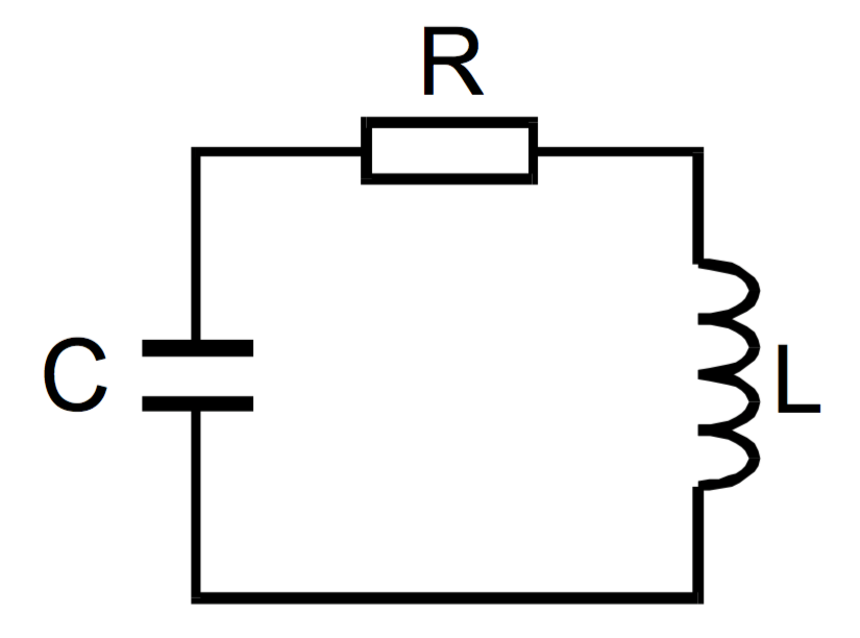
\includegraphics[height = 3 cm]{RCL.pdf}
  \caption{Eine \textbf{RCL}-Schaltung \cite{anleitung}.}
  \label{fig:rcl}
\end{figure}

Über das 2.Kirchhoffsche Gesetz, dass die Summe aller Spannungen null ist, ergibt
sich folgende Differentialgleichung:

\begin{equation}
  \frac{\symup{d}^2 \g{I}}{\symup{d t}^2} + \frac{\symup{R}}{\symup{L}}
  \frac{\g{d I}}{\g{d t}} + \frac{1}{\g{L C}} \g{I} = 0.
  \label{eqn:dgl}
\end{equation}

Als Lösungen ergeben sich die folgenden:

\begin{equation}
  \mathfrak{I}(t) = \mathfrak{U}_1 \textbf{e}^{\g{i\tilde{\omega}_1t}} + \mathfrak{U}_2
  \textbf{e}^{\g{i\tilde{\omega}_2t}}.
\end{equation}

$\mathfrak{U}_1$ und $\mathfrak{U}_2$ sind hierbei beliebige komplexe Zahlen.
$\g{\tilde{\omega}}_\text{1}$ und $\g{\tilde{\omega}}_\text{1}$ sind Konstanten nach Gleichung
\eqref{eqn:konstant}.

\begin{equation}
  \tilde{\omega}_{1,2} = \g{i\frac{R}{2 L} \pm \sqrt{\frac{1}{L C} - \frac{R^2}{4 L^2}}}
  \label{eqn:konstant}
\end{equation}

Mit den Abkürzungen

\begin{align}
  2 \pi \mu := \g{\frac{R}{2 L}} & \text{und} & 2 \pi \g{\tilde{\nu}} := \g{\sqrt{\frac{1}{L C} - \frac{R^2}{4 L^2}}}
\end{align}

ergibt sich die Gleichung \eqref{eqn:gedschw}.

\begin{equation}
  I(t) = A_0 \g{e}^{-2 \g{\pi} \mu t} \cos(2 \g{\pi} \nu t + \eta)
  \label{eqn:gedschw}
\end{equation}

Klar zu erkennen ist hier die Oszillation und die exponentielle Abnahme.
In Abbildung \ref{fig:gedschw} ist dies auch zu erkennen.

\begin{figure}[h]
  \centering
  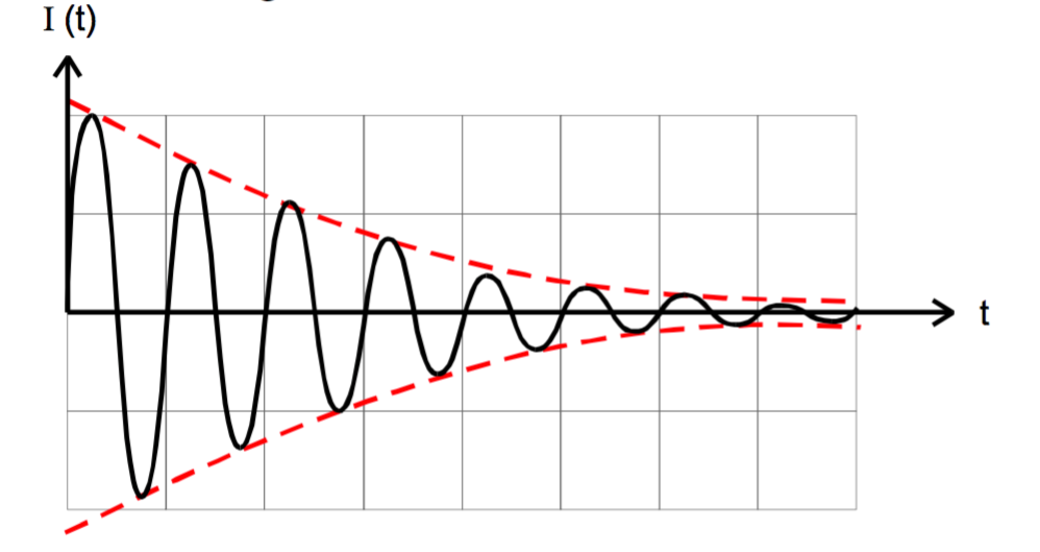
\includegraphics[width = \textwidth]{gedschw.pdf}
  \caption{Eine gedämpfte Schwingung mit der Einhüllenden $\pm e^{-2\g{\pi}\mu t}$.}
  \label{fig:gedschw}
\end{figure}
